\documentclass[fleqn,10pt]{wlscirep}
\newcommand{\autocite}[1]{\cite{#1}}
\newcommand{\textcite}[1]{\cite{#1}}

\title{Great and certainly not overstated contribution to the literature}

%%------------AUTHORS--------------
\author[1 ]{Me Ofcourse}
\author[1 ]{Some Otherdude}
\author[2 ,$\ast$ ]{And Thisguy}

\affil[1]{Institute for Psychology, University of Tromsø}
\affil[2]{University of Otherplace}

\affil[*]{and.thisguy@otherplace.org}
%%------------/AUTHORS--------------


\keywords{
latex,
markdown,
}
%\keywords{Keyword1, Keyword2, Keyword3}

\begin{abstract}
%% Text of abstract
Lorem ipsum dolor sit amet, consectetur adipiscing elit, sed do eiusmod
tempor incididunt ut labore et dolore magna aliqua. Ut enim ad minim
veniam, quis nostrud exercitation ullamco laboris nisi ut aliquip ex ea
commodo consequat. Duis aute irure dolor in reprehenderit in voluptate
velit esse cillum dolore eu fugiat nulla pariatur. Excepteur sint
occaecat cupidatat non proident, sunt in culpa qui officia deserunt
mollit anim id est laborum.

Lorem ipsum dolor sit amet, consectetur adipiscing elit, sed do eiusmod
tempor incididunt ut labore et dolore magna aliqua. Ut enim ad minim
veniam, quis nostrud exercitation ullamco laboris nisi ut aliquip ex ea
commodo consequat. Duis aute irure dolor in reprehenderit in voluptate
velit esse cillum dolore eu fugiat nulla pariatur. Excepteur sint
occaecat cupidatat non proident, sunt in culpa qui officia deserunt
mollit anim id est laborum.
\end{abstract}


\begin{document}

\flushbottom
\maketitle
% * <john.hammersley@gmail.com> 2015-02-09T12:07:31.197Z:
%
%  Click the title above to edit the author information and abstract
%
\thispagestyle{empty}

%\noindent Please note: Abbreviations should be introduced at the first mention in the main text – no abbreviations lists. Suggested structure of main text (not enforced) is provided below.

%% main text
\hypertarget{introduction}{%
\section{Introduction}\label{introduction}}

Lorem ipsum dolor sit amet, consectetur adipiscing elit, sed do eiusmod
tempor incididunt ut labore et dolore magna aliqua. Ut enim ad minim
veniam, quis nostrud exercitation ullamco laboris nisi ut aliquip ex ea
commodo consequat. Duis aute irure dolor in reprehenderit in voluptate
velit esse cillum dolore eu fugiat nulla pariatur. Excepteur sint
occaecat cupidatat non proident, sunt in culpa qui officia deserunt
mollit anim id est laborum.

References are cited as \textcite{mittner2014brain} or
\autocite{mittner2014brain}.

\hypertarget{methods}{%
\section{Methods}\label{methods}}

Footnotes can be entered using this code\footnote{a footnote}.

Figures are included like this.

\begin{figure}
\centering
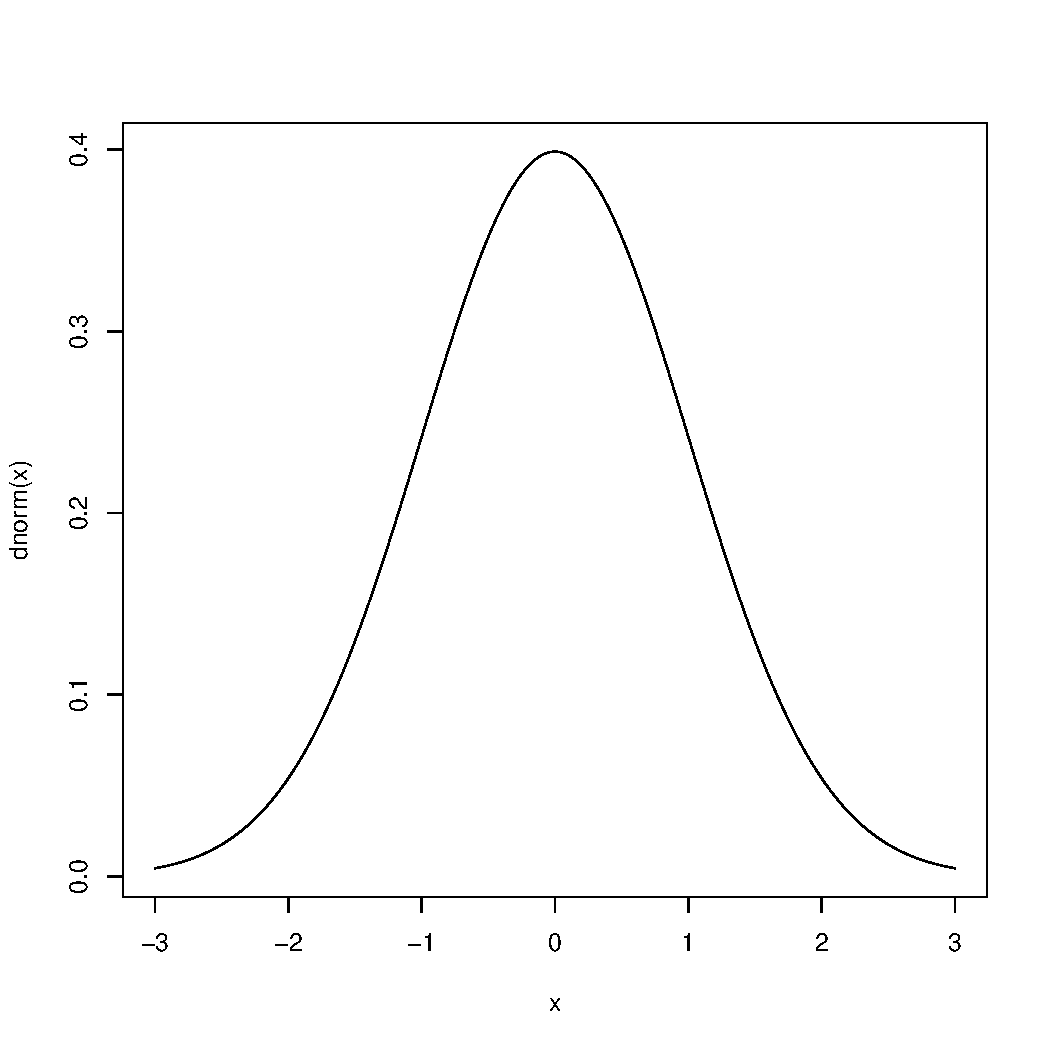
\includegraphics{pics/dummy.pdf}
\caption{This is gonna be the caption.\label{fig:dummy}}
\end{figure}

And referenced from here as Fig. \ref{fig:dummy}.

Complex tables can use standard LaTeX code as this one.

Equations can be used inline \(y=\beta_0 + \beta_1 x + \epsilon\) or as
usual \[f(x)=\frac{1}{x}\]

\begin{table}[ht]
\centering
\caption{Probability to observe Bayes Factors of a certain magnitude or above for the used sample-size of $N=60$ assuming the original and the null-hypothesis.}
\begin{tabular}{llrrr}
  & & \multicolumn{3}{l}{$P(\text{BF}\ge\theta)$}\\
  Hypothesis & BF Type & $\theta=3$ & $\theta=10$ & $\theta=20$ \\
  \hline
  $d\sim \mathcal{N}(1.57, 0.51)$ & JZS BF$_{10}$ & 0.98 & 0.97 & 0.96 \\
     & Replication BF$_{10}$ & 0.98 & 0.96 & 0.96 \\
     & Meta-Analysis BF$_{10}$ & 0.99 & 0.99 & 0.99 \\\cline{2-5}
    $d=0$ & JZS BF$_{01}$ & 0.81 & 0.00 & 0.00 \\
   & Replication BF$_{01}$ & 0.98 & 0.95 & 0.91 \\
     & Meta-Analysis BF$_{01}$ & 0.63 & 0.27 & 0.06 \\
   \hline
\end{tabular}
\label{tab:probbf}
\end{table}

\hypertarget{results}{%
\section{Results}\label{results}}

\hypertarget{discussion}{%
\section{Discussion}\label{discussion}}

\bibliography{references.bib}

\section*{Acknowledgements}
We'd like to thank bla bla and blablab

\section*{Author contributions statement}
Must include all authors, identified by initials, for example: A.A.
conceived the experiment(s), A.A. and B.A. conducted the experiment(s),
C.A. and D.A. analysed the results. All authors reviewed the manuscript.


\section*{Additional information}
To include, in this order: \textbf{Accession codes} (where applicable);
\textbf{Competing financial interests} (mandatory statement). The
corresponding author is responsible for submitting a
\href{http://www.nature.com/srep/policies/index.html#competing}{competing financial interests statement}
on behalf of all authors of the paper. This statement must be included
in the submitted article file.
To include, in this order: \textbf{Accession codes} (where applicable);
\textbf{Competing financial interests} (mandatory statement). The
corresponding author is responsible for submitting a
\href{http://www.nature.com/srep/policies/index.html#competing}{competing financial interests statement}
on behalf of all authors of the paper. This statement must be included
in the submitted article file.

\end{document}
